%\documentstyle[epsf,twocolumn]{jarticle}       %LaTeX2e仕様
\documentclass[twocolumn]{jarticle}     %pLaTeX2e仕様(platex.exeの場合)
% \documentclass[onecolumn]{ujarticle}   %pLaTeX2e仕様(uplatex.exeの場合)
%%%%%%%%%%%%%%%%%%%%%%%%%%%%%%%%%%%%%%%%%%%%%%%%%%%%%%%%%%%%%%
%%
%%  基本バージョン
%%
%%%%%%%%%%%%%%%%%%%%%%%%%%%%%%%%%%%%%%%%%%%%%%%%%%%%%%%%%%%%%%%%
\setlength{\topmargin}{-45pt}
%\setlength{\oddsidemargin}{0cm}
\setlength{\oddsidemargin}{-7.5mm}
%\setlength{\evensidemargin}{0cm}
\setlength{\textheight}{24.1cm}
%setlength{\textheight}{25cm}
\setlength{\textwidth}{17.4cm}
%\setlength{\textwidth}{172mm}
\setlength{\columnsep}{11mm}

%\kanjiskip=.07zw plus.5pt minus.5pt


% 【節が変わるごとに (1.1)(1.2) … (2.1)(2.2) と数式番号をつけるとき】
%\makeatletter
%\renewcommand{\theequation}{%
%\thesection.\arabic{equation}} %\@addtoreset{equation}{section}
%\makeatother

%\renewcommand{\arraystretch}{0.95} 行間の設定
%%%%%%%%%%%%%%%%%%%%%%%%%%%%%%%%%%%%%%%%%%%%%%%%%%%%%%%%
%\usepackage{graphicx}   %pLaTeX2e仕様(\documentstyle ->\documentclass)
\usepackage[dvipdfmx]{graphicx}
\usepackage{subcaption}
\usepackage{multirow}
\usepackage{amsmath}
\usepackage{url}
\usepackage{ulem}
\usepackage{algorithm}
\usepackage{algorithmic}
\usepackage{listings} %,jlisting} %日本語のコメントアウトをする場合jlistingが必要
%ここからソースコードの表示に関する設定
\lstset{
  basicstyle={\ttfamily},
  identifierstyle={\small},
  commentstyle={\smallitshape},
  keywordstyle={\small\bfseries},
  ndkeywordstyle={\small},
  stringstyle={\small\ttfamily},
  frame={tb},
  breaklines=true,
  columns=[l]{fullflexible},
  numbers=left,
  xrightmargin=0zw,
  xleftmargin=3zw,
  numberstyle={\scriptsize},
  stepnumber=1,
  numbersep=1zw,
  lineskip=-0.5ex
}
%%%%%%%%%%%%%%%%%%%%%%%%%%%%%%%%%%%%%%%%%%%%%%%%%%%%%%%%
\begin{document}

	%bibtex用の設定
	%\bibliographystyle{ujarticle}

	\twocolumn[
		\noindent
		\hspace{1em}
		2020 年 10 月 16 日
		ゼミ資料
		\hfill
		B4 杉山 竜弥
		\vspace{2mm}

		\hrule
		\begin{center}
			{\Large \bf 進捗報告}
		\end{center}
		\hrule
		\vspace{9mm}
	]

	% ‚ここから 文章 Start!
% \section{今週やったこと}
% \begin{itemize}
% 	\item グラフ距離の計算
% \end{itemize}

\section{今週やったこと}
\begin{itemize}
  \item 10回の探索実験
  \item optunaでscheduler最適化
\end{itemize}

\section{実験}

統計的な評価を得るため, 探索実験を複数回行った.

\begin{table}[tb]
  \begin{center}
    \caption{実験の設定}
    \begin{tabular}{|c|c|} \hline
      base model & VGG19 \\ \hline
      Optim($w$) & SGD(lr=0.01, momentum=0.9) \\ \hline
      Optim($\alpha$) & Adam(lr=0.005, $\beta$=(0.5, 0.999)) \\ \hline
      Loss & Cross Entropy Loss \\ \hline
      dataset & cifar10 \\ \hline
      batch size & 64 \\ \hline
    \end{tabular}
    \label{tab:setting}
  \end{center}
\end{table}

表\ref{tab:setting}に探索時の実験設定を示した.

\subsection{結果}

% \begin{figure}[tb]
% 	\begin{center}
% 		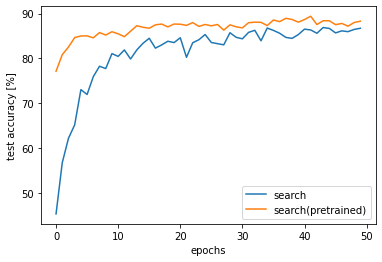
\includegraphics[clip,width=75mm]{acc.png}
% 		\caption{学習中のテスト精度}
% 		\label{fig:acc}
% 	\end{center}
% \end{figure}


\section{実験}

schedulerの探索をoptunaでした.
表\ref{tab:setting2}, \ref{tab:res}にoptunaの実験設定を示した.

\begin{table}[tb]
  \begin{center}
    \caption{実験2の設定}
    \begin{tabular}{|c|c|} \hline
      model & VGG19 \\ \hline
      Optim & SGD(momentum=0.9) \\ \hline
      Loss & Cross Entropy Loss \\ \hline
      dataset & cifar10 \\ \hline
      train size & 2000 \\ \hline
      epoch & 100 \\ \hline
      batch size & 64 \\ \hline
    \end{tabular}
    \label{tab:setting2}
  \end{center}
\end{table}

\begin{table}[tb]
  \begin{center}
    \caption{optunaの設定と結果}
    \begin{tabular}{|c|c|c|} \hline
      変数       & 探索空間                                                        & best     \\ \hline
      lr       & 0.1 $\sim$0.0001                                            & 0.000101 \\ \hline
      schduler & \begin{tabular}[c]{@{}c@{}}step,\\ exponential\end{tabular} & step     \\ \hline
      step     & 30, 40, ... , 100                                           & 40       \\ \hline
    \end{tabular}
    \label{tab:res}
  \end{center}
\end{table}

\section{考察}
optunaは時間がかかるので, 設定を最適化するoptunaをうまく回す設定も難しい.

\section{今後の予定}
% なんとなくなんかの勉強をするとかではなく具体的に
optunaの結果から得た設定で, 評価段階の実験を10回行い, 統計的な性能を評価する.
% \begin{itemize}
  % \item 重みと編集距離の変化の調査
  % \item DARTのunrolling実験
% \end{itemize}

\section{ソースコード}
% 埋め込みでもGitでもいいので参照できるように
githubのnotebookリポジトリ参照.

% 参考文献リスト
\bibliographystyle{unsrt}
\bibliography{ref}
\end{document}
